\documentclass[10pt,a4paper]{article}
\usepackage{amssymb}
\usepackage[left=2.25cm,right=2.25cm,top=2.25cm,bottom=2.75cm]{geometry}
\usepackage{graphicx}
\usepackage{isabelle}
\usepackage{isabellesym}
\usepackage[only,bigsqcap]{stmaryrd}
\usepackage{pdfsetup}

\urlstyle{tt}
\isabellestyle{it}

% for uniform font size
%\renewcommand{\isastyle}{\isastyleminor}

\renewcommand{\isacharunderscore}{\_}

\begin{document}

\title{Formalization of Bachmair and Ganzinger's \\ Ordered Resolution Prover}
\author{Anders Schlichtkrull, Jasmin Christian Blanchette, Dmitriy Traytel, and Uwe Waldmann}

\maketitle

\begin{abstract}
\noindent
This Isabelle/HOL formalization covers Sections 2 to 4 of Bachmair and
Ganzinger's ``Resolution Theorem Proving'' chapter in the \emph{Handbook of
Automated Reasoning}. This includes soundness and completeness of unordered
and ordered variants of ground resolution with and without literal selection,
the standard redundancy criterion, a general framework for refutational
theorem proving, and soundness and completeness of an abstract first-order
prover.
\end{abstract}

\tableofcontents

% sane default for proof documents
\parindent 0pt
\parskip 0.5ex

\section{Introduction}

Bachmair and Ganzinger's ``Resolution Theorem Proving'' chapter
%\cite{bachmair-ganzinger-2001}
in the \emph{Handbook of Automated Reasoning} is the standard reference on the
topic. It defines a general framework for propositional and first-order
resolution-based theorem proving. Resolution forms the basis for
superposition, the calculus implemented in many popular automatic theorem
provers.

\medskip

This Isabelle/HOL formalization covers Sections 2.1, 2.2, 2.4, 2.5, 3, 4.1,
4.2, and 4.3 of Bachmair and Ganzinger's chapter. Section 2 focuses on
preliminaries. Section 3 introduces unordered and ordered variants of ground
resolution with and without literal selection and proves them refutationally
complete. Section 4.1 presents a framework for theorem provers based on
refutation and saturation. Section 4.2 generalizes the refutational
completeness argument and introduces the standard redundancy criterion, which
can be used in conjunction with ordered resolution. Finally, Section 4.3 lifts
the result to a first-order prover, specified as a calculus.
Figure~\ref{fig:thys} shows the corresponding Isabelle theory structure.

\medskip

We refer to the following publications for details:

\begin{quote}
Anders Schlichtkrull, Jasmin Christian Blanchette, Dmitriy Traytel, Uwe Waldmann: \\
Formalizing Bachmair and Ganzinger's Ordered Resolution Prover. \\
IJCAR 2018: 89-107 \\
\url{http://matryoshka.gforge.inria.fr/pubs/rp_paper.pdf}

\medskip

Anders Schlichtkrull, Jasmin Blanchette, Dmitriy Traytel, Uwe Waldmann: \\
Formalizing Bachmair and Ganzinger's Ordered Resolution Prover. \\
Journal of Automated Reasoning \\
\url{http://matryoshka.gforge.inria.fr/pubs/rp_article.pdf}
\end{quote}

\begin{figure}
\begin{center}
  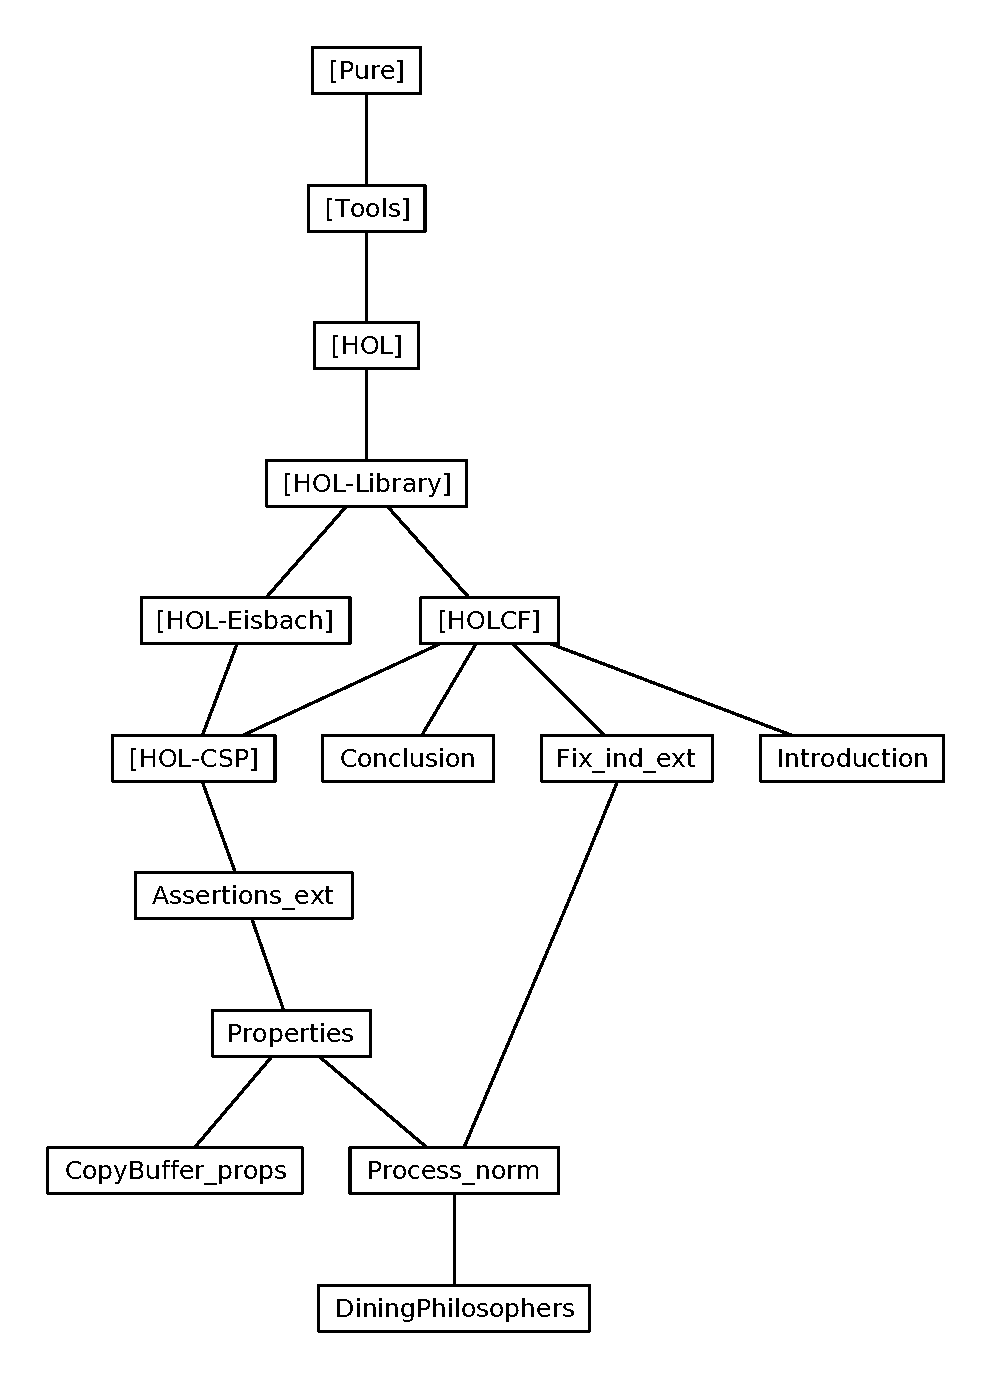
\includegraphics[width=0.75\textwidth,keepaspectratio]{session_graph}
\end{center}
\caption{Theory dependency graph}
\label{fig:thys}
\end{figure}

% generated text of all theories
\input{session}

% optional bibliography
% \bibliographystyle{abbrv}
% \bibliography{bib}

\end{document}
